%% ICAIF '26 poster for "Making Tail Constraints Bind" (paper 873).
%% A0 portrait (84.1 x 118.9 cm), as required by the organisers.
%% Style follows the Columbia MAFN posters: full-width blue title banner with
%% logos, two plain columns, centred bold section headings, sans-serif text.
%% Build: cd poster && latexmk -pdf poster.tex
%% Figures are the paper's vector PDFs. Logos live in logos/.
\documentclass[25pt, a0paper, portrait, margin=0mm, innermargin=25mm,
  blockverticalspace=10mm, colspace=25mm, subcolspace=8mm]{tikzposter}

\usepackage[T1]{fontenc}
\usepackage{amsmath}
\usepackage[scaled=0.95]{helvet}
\renewcommand{\familydefault}{\sfdefault}
\usepackage{sfmath}
\usepackage{booktabs}
\usepackage{graphicx}
\usepackage{qrcode}
\usepackage{fontawesome5}
\usepackage{enumitem}
\usepackage{ragged2e}
\usetikzlibrary{arrows.meta, positioning, calc}
\graphicspath{{../paper/figures/}{logos/}}

%% ---------------------------------------------------------------------------
%% Palette. The banner is the MAFN crown's blue, so the crown tile blends in.
%% Navy for headings and highlights matches scripts/_paper_style.py.
\definecolor{ink}{HTML}{222222}
\definecolor{navy}{HTML}{2F4B7C}
\definecolor{banner}{HTML}{013088}
\definecolor{dark}{HTML}{4D4D4D}
\definecolor{mid}{HTML}{8C8C8C}
\colorlet{tint}{navy!7}

\usetheme{Default}
\usetitlestyle{Filled}
\colorlet{backgroundcolor}{white}
\colorlet{framecolor}{white}
\colorlet{titlefgcolor}{white}
\colorlet{titlebgcolor}{banner}
\colorlet{blocktitlebgcolor}{white}
\colorlet{blocktitlefgcolor}{navy}
\colorlet{blockbodybgcolor}{white}
\colorlet{blockbodyfgcolor}{ink}

%% Sections: centred bold heading, no frame or fill.
\defineblockstyle{Plain}{
  titlewidthscale=1, bodywidthscale=1, titlecenter,
  titleoffsetx=0pt, titleoffsety=0pt, bodyoffsetx=0pt, bodyoffsety=0pt,
  bodyverticalshift=0pt, roundedcorners=0, linewidth=0pt,
  titleinnersep=3mm, bodyinnersep=3mm
}{}
\useblockstyle{Plain}
\tikzposterlatexaffectionproofoff

%% ---------------------------------------------------------------------------
\newcommand{\hl}[1]{\textcolor{navy}{\textbf{#1}}}
\newcommand{\iconitem}[1]{\hangindent=1.5em\hangafter=1\noindent
  \makebox[1.5em][l]{\textcolor{navy}{\faCheckSquare[regular]}}#1}
\newcommand{\diag}[1]{\par\smallskip\noindent{\setlength{\fboxsep}{5mm}\colorbox{tint}{%
  \begin{minipage}{\dimexpr\linewidth-10mm}\RaggedRight\iconitem{#1}\end{minipage}}}\par}
\newcommand{\fig}[2][0.78\linewidth]{\par\medskip{\centering
  \includegraphics[width=#1]{#2}\par}}
\newcommand{\figcap}[1]{{\centering\small\color{dark}#1\par}\medskip}
\setlist{leftmargin=1.1em, itemsep=2mm, topsep=2mm, label=\textcolor{navy}{\textbullet},
  before=\RaggedRight}
\setlength{\parskip}{0.45em}
%% Block bodies default to \large; set them one step down for this text density.
\newcommand{\body}{\fontsize{26.5}{32.5}\selectfont\setlength{\parskip}{0.45em}}

\newcommand{\repourl}{https://github.com/nl2992/ICAIF_cvar-rl-portfolio-allocator}

%% ---------------------------------------------------------------------------
\settitle{%
  \begin{minipage}[c]{0.14\linewidth}\centering
    
\includegraphics[height=58mm]{logos/mafn.png}\par\vspace{6mm}
    
\includegraphics[height=70mm]{logos/unsw.png}
  \end{minipage}\hfill
  \begin{minipage}[c]{0.70\linewidth}\centering\color{white}
    {\fontsize{70}{84}\selectfont\bfseries Making Tail Constraints Bind: Two Silent Failure
      Modes in CVaR-Constrained Portfolio RL\par}
    \vspace{10mm}
    {\LARGE Nigel Li$^{1,2}$\qquad Yutong Han$^{2}$\par}
    \vspace{4mm}
    {\large\itshape $^1$University of New South Wales, Sydney\qquad
      $^2$Columbia University, New York City\par}
  \end{minipage}\hfill
  \begin{minipage}[c]{0.14\linewidth}\centering
    
\includegraphics[width=\linewidth]{logos/icaif_white.png}
  \end{minipage}}

\begin{document}
\maketitle[innersep=14mm, titletoblockverticalspace=14mm]

\begin{columns}
%% ===========================================================================
\column{0.5}
\block{Abstract}{\body
  Train a portfolio allocator with reinforcement learning (RL) to maximise return and it has
  no reason to avoid big losses. The usual fix is a Lagrangian penalty on Conditional
  Value-at-Risk (CVaR), the average loss in the worst weeks. We found two ways this fix can
  quietly do nothing. If the penalty and the reward are on different scales, the penalty
  weight stays at zero and the budget is never enforced, yet the tail numbers still improve,
  so the problem is easy to miss. And the choice of test can decide the winner, because a
  single stress window and a rolling walk-forward rank the same methods in opposite order.
  Our answer is a filter that checks each portfolio before it trades and moves it toward
  minimum variance when its forecast CVaR is over budget. Out of sample, the share of weeks
  over budget falls from \hl{75.1\% to 7.4\%}. Across 40 walk-forward folds on two
  universes, the constraint lowers tail risk in \hl{26 of the 27} folds where it binds
  ($p=8.8\times10^{-6}$).
}

\block{Why a Tail Limit}{\body
  In the week of 16 March 2020 the S\&P 500 fell about 15\% and the VIX closed at a record
  82.69. Our allocator trained only for return was still holding equities. The same allocator
  with a CVaR limit had already moved into Treasuries and cash, and its drawdown was
  \hl{7.7\% against 16.3\%}.
  \fig[0.9\linewidth]{figure_stress_paths.pdf}
  \figcap{Figure 1. Drawdown over 2020--2024. Bold lines are the five-seed average.}
}

\block{How the Allocator Works}{\body
  Every week the allocator splits money across seven ETFs that cover the main macro blocks
  (SPY, TLT, HYG, DBC, GLD, UUP, BIL). It is long-only, holds at most 40\% in any one asset,
  has its weekly turnover capped at 0.50 and pays 5\,bps per trade. We use 887 weekly returns
  from 2008 to 2024. The budget caps $\mathrm{CVaR}_{0.95}$, the average loss in the worst 5\%
  of weeks, at $d=1.2\%$. Training back-propagates straight through the portfolio return.
  \[
    \mathcal{L} = -\mathrm{Sharpe} + \lambda\,\mathrm{ReLU}\big(\widehat{\mathrm{CVaR}}-d\big)
      + \kappa\,\mathrm{turnover},\qquad
    \lambda \leftarrow \max\{0,\ \lambda + \eta_\lambda(\widehat{\mathrm{CVaR}}-d)\}
  \]
  \vspace{2mm}
  \centering
  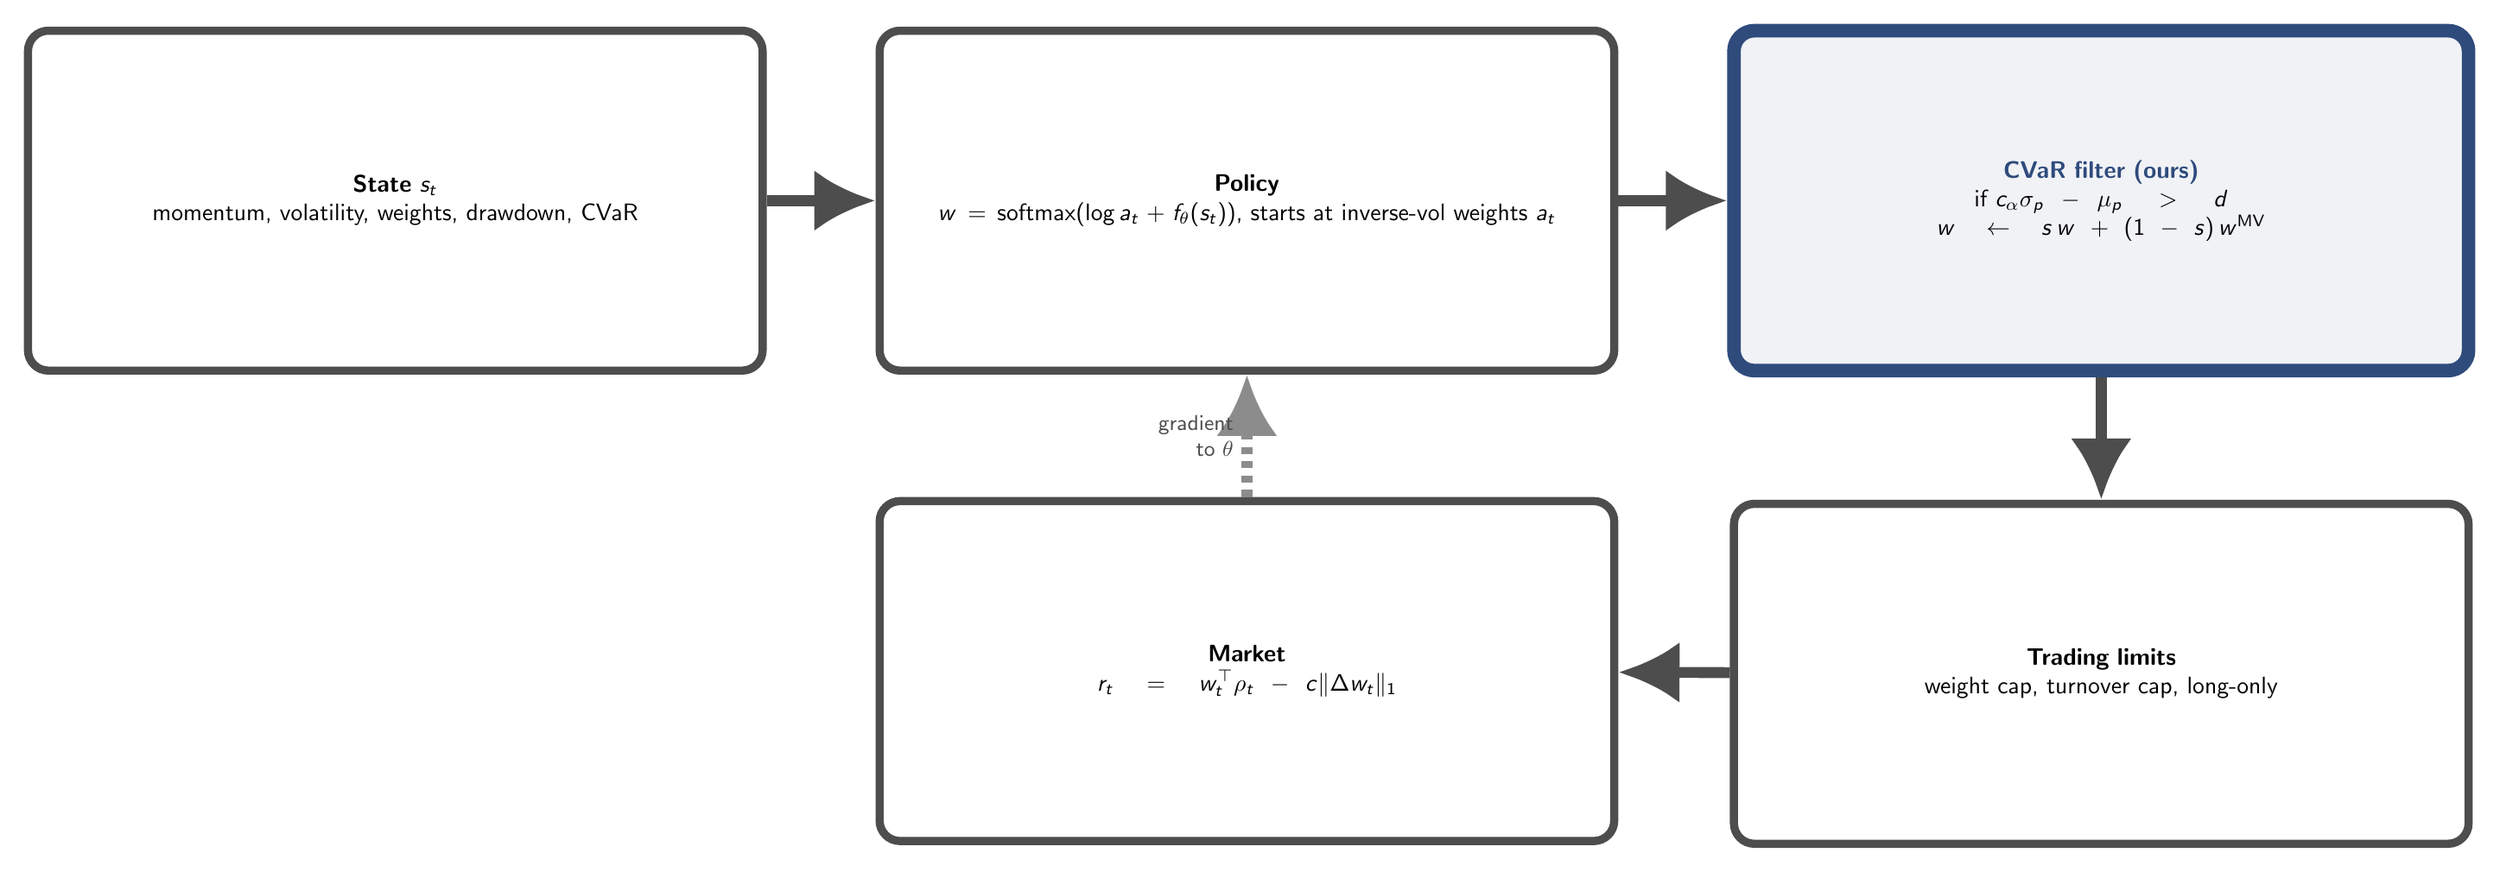
\begin{tikzpicture}[
      box/.style={draw=dark, line width=1.2mm, rounded corners=3mm, align=center,
        text width=100mm, minimum height=50mm, inner sep=4mm, font=\normalsize, fill=white},
      ours/.style={box, draw=navy, fill=tint, line width=2mm},
      arr/.style={-{Latex[length=9mm, width=9mm]}, line width=1.6mm, color=dark},
      node distance=18mm and 16mm]
    \node[box] (s) {\textbf{State $s_t$}\\ momentum, volatility, weights, drawdown, CVaR};
    \node[box, right=of s] (a) {\textbf{Policy}\\
      $w=\mathrm{softmax}(\log a_t + f_\theta(s_t))$, starts at inverse-vol weights $a_t$};
    \node[ours, right=of a] (f) {\textbf{\color{navy}CVaR filter (ours)}\\
      if $c_\alpha\sigma_p-\mu_p>d$\\ $w \leftarrow s\,w + (1-s)\,w^{\mathrm{MV}}$};
    \node[box, below=of f] (p) {\textbf{Trading limits}\\ weight cap, turnover cap, long-only};
    \node[box, below=of a] (m) {\textbf{Market}\\ $r_t = w_t^{\top}\rho_t - c\lVert\Delta w_t\rVert_1$};
    \draw[arr] (s) -- (a);
    \draw[arr] (a) -- (f);
    \draw[arr] (f) -- (p);
    \draw[arr] (p) -- (m);
    \draw[arr, color=mid, dashed] (m.north) -- node[left, font=\small, text=dark,
      align=right] {gradient\\ to $\theta$} (a.south);
  \end{tikzpicture}
  \par\RaggedRight\smallskip
  {\small\color{dark} The filter estimates CVaR from the last 104 weeks of returns (Gaussian,
  $c_{0.95}=2.06$) and keeps as much of the original portfolio as the budget allows. It only
  sees data up to the previous week, and a test confirms it cannot see the future.\par}
}

\block{Failure 1. The Penalty Never Switches On}{\body
  The penalty weight $\lambda$ is supposed to rise whenever the portfolio is over budget. In
  our setup the CVaR overshoot is around $10^{-2}$, and with a step size of $10^{-3}$ each
  update nudges $\lambda$ by about $10^{-5}$. After 1500 updates it has barely moved. A
  model-free actor--critic did the same thing when its reward signal was standardised and its
  cost signal was left at $10^{-3}$.
  \fig[0.9\linewidth]{figure_lambda_trace.pdf}
  \figcap{Figure 2. $\lambda$ during training. Bold lines are the five-seed average.}
  Why is this easy to miss? The rest of the pipeline cuts $\mathrm{CVaR}_{99}$ by \hl{61\%}
  on its own, even with $\lambda$ near zero ($p=0.0044$). The tail numbers look good whether
  or not the penalty is doing anything.
  \diag{\textbf{Check this.} Plot $\lambda$ during training. If it sits at zero, the
  constraint is switched off.}
}

%% ===========================================================================
\column{0.5}
\block{Failure 2. The Test Picks the Winner}{\body
  On a 31-asset universe, a single stress test makes our learner look better than every
  classical optimiser (Sharpe 0.85 against 0.23 for minimum variance). Run the same comparison
  as a 20-fold rolling walk-forward and minimum variance comes out well ahead (1.40 against
  0.74). Better covariance estimates (Ledoit--Wolf) do not explain the gap. The tail-risk
  benefit over unconstrained RL shows up under both tests ($p=6\times10^{-4}$). The win over
  the optimiser shows up in only one.
  \fig[0.6\linewidth]{figure_protocol.pdf}
  \figcap{Figure 3. The same four methods ranked by two different tests.}
  \diag{\textbf{Check this.} Compare learners with optimisers on rolling walk-forward folds
  and report Deflated Sharpe, not one test window.}
}

\block{The Fix. Check Every Trade}{\body
  A larger step size makes the penalty work during training, but not on new data. The
  portfolio was still over budget in 75\% of test weeks, and four different ways of setting
  the budget all landed between 71\% and 78\%. So instead of relying on the penalty alone, we
  added a check right before each trade.
  \fig[0.62\linewidth]{figure_filter_frontier.pdf}
  \figcap{Figure 4. Share of weeks over budget against Sharpe. The dashed line is the 5\% we
  allow.}
  \centering
  \begin{tabular}{@{}lrrr@{}}
    \toprule
    variant (5-seed mean) & Sharpe & $\mathrm{CVaR}_{99}$ & over budget \\
    \midrule
    A1 no constraint & 0.626 & 0.065 & 100.0\% \\
    A2 penalty, step too small & 0.987 & 0.025 & 7.9\% \\
    A3 penalty, step fixed & 0.911 & 0.028 & 75.1\% \\
    A7 penalty adjusted live & 0.826 & 0.031 & 81.9\% \\
    \hl{A6 filter + penalty} & \hl{0.851} & \hl{0.016} & \hl{7.4\%} \\
    \midrule
    minimum variance & 0.901 & & 7.9\% \\
    \bottomrule
  \end{tabular}
  \par\RaggedRight\smallskip
  A7 keeps raising $\lambda$ during testing and is still over budget, so A6's gain comes
  from the filter.
}

\block{Does It Hold Up?}{\body
  We re-ran the comparison as a rolling walk-forward with 26-week test windows on two
  universes, measuring $\mathrm{CVaR}_{99}$ with and without the constraint.
  \par\medskip\centering
  \begin{tabular}{@{}lrrr@{}}
    \toprule
    universe & folds & lower tail risk & Wilcoxon $p$ \\
    \midrule
    macro ETFs (7) & 20 & 9 (11 tied) & 0.0077 \\
    sector ETFs (10) & 20 & 17 & 0.0003 \\
    \hl{pooled} & \hl{40} & \hl{26 of 27 untied} & \hl{$8.8\times10^{-6}$} \\
    grouped by calendar & 20 & & $3.3\times10^{-4}$ \\
    \bottomrule
  \end{tabular}
  \par\RaggedRight\smallskip
  A tie is a fold where the budget never binds, so both versions hold the same portfolio.
  Both universes pass a Benjamini--Hochberg correction. Re-running the stress test on sector
  ETFs gives the same picture, with $\mathrm{CVaR}_{99}$ down 30\% and Sharpe unchanged.
}

\block{Limitations and Takeaways}{\body
  Our learner does not beat plain rolling minimum variance on Sharpe out of sample. Once you
  correct for the number of configurations tried (Deflated Sharpe), its Sharpe edge over
  classical rules disappears. What does hold up is lower tail risk and staying within budget.
  We only tested weekly data with simple trading costs, and the Gaussian forecast in the
  filter can underestimate fat tails. If you build one of these, four checks are worth doing.
  \par\smallskip
  \iconitem{\textbf{Plot $\lambda$.} A flat line at zero means the constraint is off.}\par
  \iconitem{\textbf{Put reward and cost on the same scale.} Standardise the cost signal and
    size the step to the CVaR overshoot.}\par
  \iconitem{\textbf{Test on rolling folds} and report Deflated Sharpe before claiming you
    beat an optimiser.}\par
  \iconitem{\textbf{Enforce the budget when you trade.} A penalty only discourages breaches
    on average.}\par
  \medskip
  \begin{minipage}[c]{0.83\linewidth}\RaggedRight\footnotesize\color{dark}
    Rockafellar \& Uryasev 2000. Altman 1999. Stooke et al.\ 2020. Ji et al.\ 2024.
    Dalal et al.\ 2018. Bailey \& L\'opez de Prado 2014.\par
    \faEnvelope[regular]\ nigel.li@unsw.edu.au \quad yh3915@columbia.edu\par
    \faGithub\ github.com/nl2992/ICAIF\_cvar-rl-portfolio-allocator
  \end{minipage}\hfill
  \begin{minipage}[c]{0.14\linewidth}\centering
    \qrcode[height=\linewidth]{\repourl}
  \end{minipage}
}
\end{columns}

\end{document}
